\documentclass[journal]{IEEEtran}

\usepackage{amsmath,amssymb,amsfonts}
\usepackage{amsthm}
\usepackage{graphicx}
\usepackage{booktabs}
\usepackage{array}
\usepackage{cite}
\usepackage{url}
\usepackage[caption=false,font=footnotesize]{subfig}

\newtheorem{lemma}{Lemma}
\newtheorem{theorem}{Theorem}
\newtheorem{remark}{Remark}

\newcommand{\Qtol}{Q_{\mathrm{tol}}}
\newcommand{\epssec}{\varepsilon_{\mathrm{sec}}}
\newcommand{\epscor}{\varepsilon_{\mathrm{cor}}}
\newcommand{\fEC}{f_{\mathrm{EC}}}
\newcommand{\leakEC}{\mathrm{leak}_{\mathrm{EC}}}
\newcommand{\ech}{e_{\mathrm{ch}}}
\newcommand{\Nmin}{N_{\min}}

\graphicspath{{figures/}}

\begin{document}

\title{Finite-Key Security Analysis of the BB84 Quantum Key Distribution Protocol under Intercept-Resend Attacks and Quantum Channel Noise}

\author{Author~One,~\IEEEmembership{Member,~IEEE,}
        Author~Two,
        and~Author~Three%
\thanks{Manuscript received XX XX, 2026; revised XX XX, 2026.
The authors are with the Department of XXXX, University of XXXX, City, Country
(e-mail: author@example.edu).}}

\markboth{IEEE Transactions / Journal Name, Vol.~XX, No.~X, Month~2026}%
{Author \MakeLowercase{\textit{et al.}}: Finite-Key Security of BB84 under Intercept-Resend Attacks and Channel Noise}

\maketitle

\begin{abstract}
Practical quantum key distribution (QKD) systems exchange a finite number of signals, so the asymptotic secret-key rate overestimates what can be extracted safely. This paper studies the finite-key behaviour of the BB84 protocol when the observed error statistics are generated by an intercept-resend (IR) eavesdropper that attacks a fraction $p$ of the pulses on top of a bit-flip channel with probability $\ech$. We derive the closed-form quantum bit error rate (QBER) $Q=\ech+(1-2\ech)p/4$ and combine it with a composable finite-key length bound based on the smooth min-entropy framework, in which statistical fluctuations are controlled by a Serfling-type inequality. From this we obtain the secret-key rate as a function of block length $N$, attack fraction $p$, channel noise $\ech$ and the basis bias $q_X$, the minimum block length $\Nmin$ that yields a positive key, and the largest attack fraction $p_{\max}$ that can be tolerated. A bit-level Monte Carlo simulation of the complete protocol confirms the QBER law and the predicted key rates to within statistical error, and an empirical check shows that the fluctuation bound is conservative. For $\ech=0.01$ and security parameters $\epssec=10^{-10}$, $\epscor=10^{-15}$, the protocol yields no key at $N=10^4$ once $p\ge 0.1$, tolerates $p_{\max}\approx0.26$ at $N=10^5$, and approaches the asymptotic limit $p_{\max}\approx0.36$ only for $N\gtrsim 10^8$. We also show that, for an adversary restricted to IR attacks, the general-attack bound is pessimistic, with an asymptotic tolerance of $p\approx0.58$ against $0.36$.
\end{abstract}

\begin{IEEEkeywords}
Quantum key distribution, BB84, finite-key analysis, intercept-resend attack, quantum bit error rate, privacy amplification, composable security.
\end{IEEEkeywords}

\IEEEpeerreviewmaketitle

\section{Introduction}
\IEEEPARstart{Q}{uantum} key distribution (QKD) allows two parties, Alice and Bob, to establish a shared secret key whose security rests on the laws of quantum mechanics rather than on computational assumptions. The first and still most widely deployed protocol is BB84 \cite{BB84}; its unconditional security against arbitrary attacks has been established by several independent proofs \cite{LoChau99,Mayers01,ShorPreskill00,Renner05}, and the field has been surveyed extensively \cite{Scarani09,Xu20,Pirandola20}.

Early proofs were asymptotic: they assume an infinite number of exchanged signals, so that statistical fluctuations of the observed error rate vanish. A real device exchanges a finite block of $N$ pulses within a finite time, and the parameter-estimation sample is correspondingly small. Finite-key analyses \cite{CaiScarani09,Tomamichel12,HayashiTsurumaru12,Lim14} quantify the resulting penalty in a \emph{composable} way, i.e., with explicit correctness and secrecy parameters $\epscor$ and $\epssec$. The penalty is far from negligible: key rates drop sharply for $N\lesssim 10^{6}$, and below a minimum block length no key can be generated at all.

The security theorems cited above hold against \emph{any} eavesdropper, so the key length depends only on the observed statistics. It is nevertheless instructive, and practically important for system design, to understand which statistics a specific, simple attack produces. The \emph{intercept-resend} (IR) attack is the canonical example: Eve measures each intercepted pulse in a random basis and resends her result \cite{BB84,Fuchs97}. It is easy to implement, it does not require a quantum memory, and its signature is a QBER of 25\% when applied to every pulse. In realistic links the IR statistics are superimposed on genuine channel noise, and the question of interest is how large a fraction of pulses Eve can intercept before the finite-key protocol aborts or returns a zero-length key.

\subsection{Contributions}
\begin{enumerate}
\item We derive, in closed form, the QBER of BB84 under a partial IR attack with fraction $p$ combined with an independent bit-flip channel $\ech$ (Lemma~\ref{lem:qber}).
\item We specialise the finite-key bound of Tomamichel \emph{et al.}\ \cite{Tomamichel12} to this setting, include the cost of error correction at efficiency $\fEC$, and optimise the basis bias $q_X$ at every operating point (Section~\ref{sec:analysis}).
\item We obtain the operational quantities $\Nmin(Q)$ and $p_{\max}(N,\ech)$, and relate them to the asymptotic thresholds.
\item We validate the analysis by a bit-level Monte Carlo simulation of the full protocol, and check the fluctuation bound empirically (Section~\ref{sec:results}).
\item We show that the general-attack bound is pessimistic for an IR-only adversary and quantify the gap (Remark~\ref{rem:ir}).
\end{enumerate}

\subsection{Paper Organisation}
Section~\ref{sec:related} reviews related work. Section~\ref{sec:model} defines the system, the attack model, the protocol and the security definitions. Section~\ref{sec:analysis} contains the analytical methodology. Section~\ref{sec:design} describes the simulation and the experimental design. Section~\ref{sec:results} presents the results, Section~\ref{sec:discussion} discusses limitations, and Section~\ref{sec:conclusion} concludes.

\section{Related Work}\label{sec:related}
Early finite-key analyses of BB84 relied on Chernoff- and Hoeffding-type concentration bounds \cite{Hoeffding63,CaiScarani09}. Tomamichel \emph{et al.}\ \cite{Tomamichel12} obtained a tight, composable bound using the entropic uncertainty relation for smooth entropies \cite{TomamichelRenner11} together with Serfling's inequality for sampling without replacement \cite{Serfling74}. Hayashi and Tsurumaru \cite{HayashiTsurumaru12} gave a concise analysis based on different techniques, and Lim \emph{et al.}\ \cite{Lim14} extended finite-key bounds to decoy-state QKD. Imperfect sources, such as those exploitable by photon-number-splitting attacks, are treated in \cite{GLLP04,Brassard00} and are outside the scope of this paper. Our contribution is not a new security proof, but a self-contained quantitative study of how the established finite-key bound behaves for the statistics produced by IR attacks in noisy channels, together with an independent numerical validation.

\section{System and Attack Model}\label{sec:model}

\subsection{BB84 Signal Exchange}
Alice sends $N$ pulses, each encoding a uniformly random bit $a_i\in\{0,1\}$ in a basis $\theta_i\in\{X,Z\}$. We assume an ideal single-photon source and an ideal detector without dark counts or losses; these are strong assumptions that we revisit in Section~\ref{sec:discussion}. Bob measures every pulse in a basis $\theta_i'\in\{X,Z\}$ and obtains $b_i$. Both parties choose the $X$ basis with probability $q_X\in[\tfrac12,1)$ and the $Z$ basis with probability $1-q_X$, independently. This \emph{efficient} variant of BB84 is what makes the asymptotic sifting loss vanish and is part of the protocol of \cite{Tomamichel12}.

\subsection{Intercept-Resend Attack}
Eve attacks each pulse independently with probability $p$. For an attacked pulse she measures in a uniformly random basis $\theta^{E}_i$, obtains a bit $e_i$, and sends Bob a fresh state encoding $e_i$ in basis $\theta^E_i$. If $\theta^E_i=\theta_i$, then $e_i=a_i$; otherwise $e_i$ is uniformly random and independent of $a_i$. A non-attacked pulse is forwarded unchanged.

\subsection{Channel Noise}
After Eve, each pulse passes through a channel that flips the encoded bit with probability $\ech$, independently of everything else. This is the effective bit-flip rate in the measurement bases, which also captures a depolarising channel with depolarising probability $\lambda$ via $\ech=\lambda/2$, and covers detector and alignment errors lumped into one parameter. Placing the noise after Eve corresponds to Eve being close to Alice; the QBER law below is symmetric under reordering because independent flips commute.

\subsection{Security Goal}
Following \cite{Renner05,Tomamichel12}, the protocol is $\varepsilon$-secure if it is $\epscor$-correct and $\epssec$-secret with $\epscor+\epssec\le\varepsilon$. The key is $\epscor$-correct if the probability that Alice's and Bob's final keys differ is at most $\epscor$. It is $\epssec$-secret if the joint state of the key and Eve's information is within trace distance $\epssec$ (weighted by the probability that the protocol does not abort) of an ideal, uniform, uncorrelated key.

\section{Protocol and Finite-Key Framework}\label{sec:protocol}

\subsection{Protocol Steps}
\begin{enumerate}
\item \textbf{Distribution and measurement.} $N$ pulses are exchanged as in Section~\ref{sec:model}.
\item \textbf{Sifting.} Alice and Bob publicly announce their bases. Pulses with $X$--$X$ matching form the raw key of length $n$. Pulses with $Z$--$Z$ matching, of number $k$, are used for parameter estimation. Other pulses are discarded.
\item \textbf{Parameter estimation.} They publicly compare the $k$ $Z$-basis bits and compute the observed error rate $Q_k$. If $Q_k>\Qtol$, the protocol aborts.
\item \textbf{Error correction.} One-way reconciliation \cite{BrassardSalvail93} leaks $\leakEC$ bits, modelled as $\leakEC=\fEC\,n\,h(\Qtol)$, followed by error verification with a hash of $\lceil\log_2(1/\epscor)\rceil$ bits to reach $\epscor$-correctness.
\item \textbf{Privacy amplification.} A two-universal hash function \cite{BBCM95,RennerKoenig05} compresses the corrected key to length $\ell$.
\end{enumerate}
Here $h(x)=-x\log_2x-(1-x)\log_2(1-x)$ is the binary entropy, truncated to $h(x)=1$ for $x\ge\tfrac12$ as in \cite{Tomamichel12}. The key is generated in the $X$ basis and estimated in the $Z$ basis, which is the configuration used in \cite{Tomamichel12}.

\subsection{Finite-Key Length}
The following expression is the key-length bound of \cite{Tomamichel12} for the parameter choices used here. For BB84 with perfect single photons and $q=1$ in the notation of \cite{Tomamichel12}, a secret key of length
\begin{equation}\label{eq:keylen}
\ell=\Big\lfloor n\big[1-h(\Qtol+\mu)\big]-\leakEC-2\log_2\frac1{\epssec}-\log_2\frac2{\epscor}\Big\rfloor
\end{equation}
can be extracted, where the statistical-fluctuation term is
\begin{equation}\label{eq:mu}
\mu=\sqrt{\frac{n+k}{nk}\,\frac{k+1}{k}\,\ln\frac{4}{\epssec}}.
\end{equation}
This corresponds to the choice $\varepsilon=\epssec/4$ and $\bar\varepsilon=\epssec/2$ in the optimisation over smoothing parameters in the supplementary material of \cite{Tomamichel12}, which we use instead of a numerical optimisation. The term $\mu$ is obtained by inverting a Serfling-type tail bound,
\begin{equation}\label{eq:serfling}
\Pr\big[Q_n\ge Q_k+\gamma\big]\le\exp\!\Big(-\frac{\gamma^2\,n\,k^2}{(n+k)(k+1)}\Big),
\end{equation}
where $Q_n$ denotes the (unobserved) error rate the $Z$-basis measurement would have produced on the $n$ key positions, and $Q_k$ the observed error rate on the sample. Setting the right-hand side to $\varepsilon$ gives \eqref{eq:mu}.

\begin{remark}
Equations \eqref{eq:keylen}--\eqref{eq:mu} are used as stated in \cite{Tomamichel12}; we do not re-derive the entropic uncertainty argument. All results below are therefore conditional on that theorem. The numerical value of the finite-size penalty is not an artefact of IR attacks: any attack producing the same $Q_k$ yields the same $\ell$.
\end{remark}

\section{Analytical Methodology}\label{sec:analysis}

\subsection{QBER under Intercept-Resend Attack and Channel Noise}

\begin{lemma}\label{lem:qber}
For BB84 with uniformly random Eve basis, attack fraction $p$ and independent bit-flip probability $\ech$, the QBER in both the $X$ and the $Z$ basis, conditioned on matching bases, is
\begin{equation}\label{eq:qber}
Q=\ech+(1-2\ech)\frac p4 .
\end{equation}
\end{lemma}
\begin{proof}
Consider a pulse with $\theta_i=\theta_i'$. With probability $1-p$ it is not attacked. With probability $p$ it is attacked; Eve's basis equals Alice's with probability $1/2$, in which case Eve resends the correct state, and otherwise Eve's basis differs from Alice's. In the latter case Bob measures in Alice's basis a state prepared in the conjugate basis, so his outcome is uniform and wrong with probability $1/2$. Hence the IR-induced error probability is $e_{\mathrm{IR}}=p\cdot\frac12\cdot\frac12=p/4$. The channel flips the bit independently with probability $\ech$, so the two error sources combine as the XOR of independent Bernoulli variables:
\[
Q=e_{\mathrm{IR}}(1-\ech)+(1-e_{\mathrm{IR}})\ech=\ech+e_{\mathrm{IR}}(1-2\ech),
\]
which is \eqref{eq:qber}. The argument does not depend on which basis Alice and Bob use, because Eve's basis is uniform.
\end{proof}

For $\ech=0$ and $p=1$ this gives the well-known 25\% error rate. The probability that a sample of $k$ bits reveals at least one error is $1-(1-Q)^k$, which for $\ech=0$ becomes $1-(1-p/4)^k$. Even small attacks are therefore detected with high probability for moderate $k$, but detection alone does not bound Eve's information; this is what the key length~\eqref{eq:keylen} accounts for.

\subsection{Choice of the Tolerance Threshold}
The threshold $\Qtol$ must be fixed before the protocol runs. We set
\begin{equation}\label{eq:qtol}
\Qtol=Q+z\sqrt{\frac{Q(1-Q)}{k}},\qquad z=3,
\end{equation}
where $Q$ is the value expected from \eqref{eq:qber}. This makes the probability that an honest (or merely noisy) run is aborted about $10^{-3}$, and it corresponds to a design in which the operator calibrates the expected QBER of the link. Larger $z$ lowers the abort rate at the cost of a larger $\Qtol$ and thus a shorter key.

\subsection{Expected Key Length and Optimal Basis Bias}
With $N$ pulses and bias $q_X$, the expected sizes are
\begin{equation}\label{eq:nk}
n=Nq_X^2,\qquad k=N(1-q_X)^2 .
\end{equation}
Substituting \eqref{eq:qber}, \eqref{eq:qtol} and \eqref{eq:nk} into \eqref{eq:keylen} gives $\ell(N,p,\ech,q_X)$ and the key rate $r=\ell/N$ in bits per transmitted pulse. We optimise over $q_X$ for every operating point. The trade-off is clear from \eqref{eq:mu}: increasing $q_X$ enlarges $n$ but shrinks $k$, which enlarges $\mu$ and $\Qtol-Q$. As $N\to\infty$, $q_X\to1$ and
\begin{equation}\label{eq:asym}
r_\infty=1-(1+\fEC)\,h(Q),
\end{equation}
so that no sifting loss remains. The condition $r_\infty>0$ defines the asymptotic QBER tolerance; for $\fEC=1.16$ it is $Q^\ast\approx 9.81\%$. Using \eqref{eq:qber}, the corresponding asymptotic attack tolerance is $p^\ast=4(Q^\ast-\ech)/(1-2\ech)$, i.e.\ $0.39$, $0.36$ and $0.33$ for $\ech=0$, $0.01$, $0.02$.

\subsection{Minimum Block Length and Maximum Tolerable Attack}
For a given $Q$, $\Nmin(Q)$ is the smallest $N$ for which $\max_{q_X}\ell>0$. Similarly, $p_{\max}(N,\ech)$ is the largest $p$ with $\max_{q_X}\ell>0$. Both are computed numerically by bisection; since $\ell$ is monotone in $N$ and decreasing in $p$, the bisection is well defined. At threshold the optimum is the balanced split $q_X=\tfrac12$ ($n=k$), where the fluctuation term is largest, which is why finite-size effects are so pronounced close to $Q^\ast$.

\begin{remark}[IR-only adversary]\label{rem:ir}
If Eve is \emph{known} to be restricted to the IR strategy of Section~\ref{sec:model}, one can compute her information directly. Whenever she attacks and her basis matches Alice's (a fraction $p/2$ of sifted bits) she knows $a_i$ exactly; otherwise her result is independent of $a_i$. Hence $H(A|E)=1-p/2$ per sifted bit, and the asymptotic key fraction is $1-p/2-\fEC\,h(Q)$, which vanishes at $p\approx0.594$, $0.577$, $0.560$ for $\ech=0$, $0.01$, $0.02$. This is considerably larger than the general-attack limits above. The gap is the price paid for not assuming that Eve is restricted; since a real adversary is not, the general bound \eqref{eq:keylen} is the one that provides security. The IR-only value is given only to quantify the conservatism.
\end{remark}

\section{Experimental Design}\label{sec:design}

\subsection{Simulation Methodology}
We implemented the protocol at bit level in Python (NumPy). For every trial, $N$ bits and bases are drawn for Alice and Bob; Eve's interception is simulated pulse by pulse, including her random basis and her random outcome in the wrong basis; the bit-flip channel is applied after Eve; Bob measures, the bases are sifted, $n$ and $k$ are counted, and the $Z$-sample error rate is compared to $\Qtol$. If the test passes, $\ell$ is computed from \eqref{eq:keylen} with the realised $n$ and $k$, and a rate of zero is recorded on abort. Unless noted otherwise, $\epssec=10^{-10}$, $\epscor=10^{-15}$, $\fEC=1.16$, $\ech=0.01$, $z=3$. The bias $q_X$ is set to the optimum found by the analytic search. The random seed is fixed, and the code and the per-trial raw counts are released with the manuscript.

\subsection{Experiments}
Four experiments are run.
\begin{enumerate}
\item \textbf{QBER law.} $N=10^5$, $q_X=0.8$, $60$ trials per point, $\ech\in\{0,0.02\}$, $p\in\{0,0.1,0.2,0.3,0.4,0.5,0.75,1\}$. The simulated QBER is compared with \eqref{eq:qber}.
\item \textbf{Full-protocol key rate.} $N\in\{10^4,10^5,10^6\}$ with $1500$, $200$ and $30$ trials respectively, $p\in\{0,0.1,0.2,0.3\}$, $\ech=0.01$. The simulated rate, including aborts, is compared with the analytic prediction.
\item \textbf{Analytic sweeps.} Key rate against $N$ ($60$ logarithmically spaced points from $10^{3.5}$ to $10^8$), against $p\in[0,0.6]$, and against $\ech\in[0,0.10]$; the minimum block length $\Nmin(Q)$; and the maximum tolerable attack fraction $p_{\max}$. These involve no randomness.
\item \textbf{Fluctuation-bound check.} For $(n,k)\in\{(500,500),(2000,500),(5000,1000)\}$ and $Q=0.03$, the total number of errors is drawn from a binomial distribution and split hypergeometrically, and $\Pr[Q_n-Q_k\ge\gamma]$ is estimated from $4\times10^5$ trials for comparison with \eqref{eq:serfling}.
\end{enumerate}

\section{Results}\label{sec:results}

\subsection{QBER Law}
Fig.~\ref{fig:qber} compares the simulated sifted-key QBER with \eqref{eq:qber} for $\ech\in\{0,0.02\}$ and $p\in[0,1]$, at $N=10^5$ and 60 trials per point. Agreement is within the statistical error bars (two standard deviations over trials), including the full-attack value $0.25$ at $\ech=0$ and $0.26$ at $\ech=0.02$. The $X$- and $Z$-basis error rates are statistically indistinguishable, as required by the symmetry argument in Lemma~\ref{lem:qber}. The figure also shows the asymptotic abort threshold, which an IR attack reaches at $p\approx0.39$ ($\ech=0$).

\begin{figure}[!t]
\centering
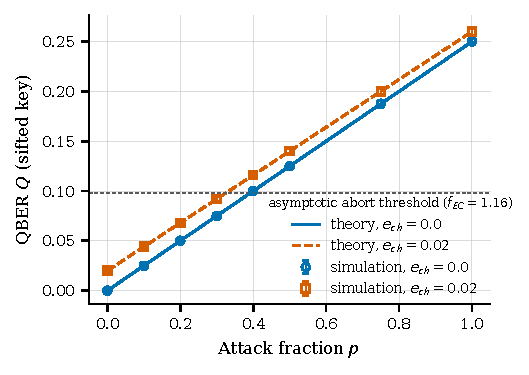
\includegraphics[width=\columnwidth]{figures/fig_qber.pdf}
\caption{Sifted-key QBER versus attack fraction $p$: theory \eqref{eq:qber} (lines) and Monte Carlo simulation (markers, $\pm2\sigma$ over trials).}
\label{fig:qber}
\end{figure}

\subsection{Key Rate versus Block Length}
Fig.~\ref{fig:rateN} shows $\ell/N$ as a function of $N$ for $\ech=0.01$ and four attack fractions, with the asymptotic limits~\eqref{eq:asym} as dotted lines. Without Eve, the first positive key appears near $N\approx5\times10^{3}$. The rate reaches $0.27$ bit/pulse at $N=10^5$, $0.45$ at $10^6$ and $0.68$ at $10^8$, against an asymptotic $0.83$. Attacks shift the whole curve to the right and flatten it: for $p=0.2$ no key exists below $N\approx4\times10^4$ and the rate is only $0.11$ bit/pulse at $N=10^6$.

\begin{figure}[!t]
\centering
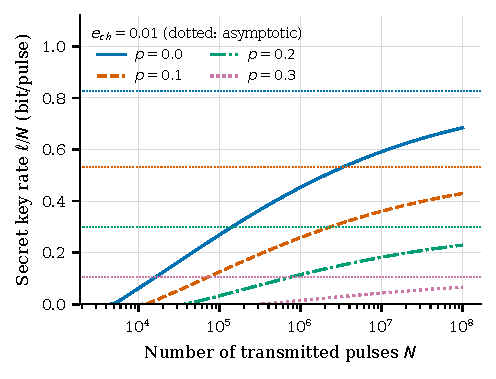
\includegraphics[width=\columnwidth]{figures/fig_rate_vs_N.pdf}
\caption{Secret-key rate versus the number of transmitted pulses for several attack fractions ($\ech=0.01$). Dotted lines: asymptotic rate \eqref{eq:asym}.}
\label{fig:rateN}
\end{figure}

Table~\ref{tab:mc} compares the full Monte Carlo protocol with the analytic prediction. The mean simulated rates agree with the analytic ones to within the trial-to-trial standard deviation in all cases, and to within $3\times10^{-4}$ bit/pulse for $N\ge10^5$. At $N=10^4$ the honest-abort probability is visible ($\approx0.3\%$), consistent with the design value of $z=3$ given the discreteness of the test statistic. At $N=10^4$ and $p\ge0.1$ the key length is non-positive, so the rate is zero by construction. The abort column for such zero-key cases reflects only the statistical test; the protocol would still terminate without key.

\begin{table}[!t]
\caption{Monte Carlo versus analytic key rate ($\ech=0.01$, $\epssec=10^{-10}$, $\epscor=10^{-15}$)}
\label{tab:mc}
\centering
\small
\begin{tabular}{@{}cccccc@{}}
\toprule
$N$ & $p$ & $q_X$ & abort (\%) & simulated $\ell/N$ & analytic \\
\midrule
$10^{4}$ & 0.0 & 0.61 & 0.27 & 0.0618 $\pm$ 0.0035 & 0.0620 \\
$10^{4}$ & 0.1 & 0.80 & 0.27 & 0.0000 $\pm$ 0.0000 & 0.0000 \\
$10^{4}$ & 0.2 & 0.80 & 0.13 & 0.0000 $\pm$ 0.0000 & 0.0000 \\
$10^{4}$ & 0.3 & 0.80 & 0.47 & 0.0000 $\pm$ 0.0000 & 0.0000 \\
$10^{5}$ & 0.0 & 0.77 & 0.00 & 0.2694 $\pm$ 0.0011 & 0.2694 \\
$10^{5}$ & 0.1 & 0.71 & 0.00 & 0.1257 $\pm$ 0.0006 & 0.1257 \\
$10^{5}$ & 0.2 & 0.61 & 0.00 & 0.0330 $\pm$ 0.0002 & 0.0330 \\
$10^{5}$ & 0.3 & 0.80 & 0.00 & 0.0000 $\pm$ 0.0000 & 0.0000 \\
$10^{6}$ & 0.0 & 0.87 & 0.00 & 0.4534 $\pm$ 0.0005 & 0.4537 \\
$10^{6}$ & 0.1 & 0.84 & 0.00 & 0.2585 $\pm$ 0.0003 & 0.2585 \\
$10^{6}$ & 0.2 & 0.79 & 0.00 & 0.1146 $\pm$ 0.0002 & 0.1147 \\
$10^{6}$ & 0.3 & 0.63 & 0.00 & 0.0148 $\pm$ 0.0000 & 0.0148 \\
\bottomrule
\end{tabular}
\end{table}


\subsection{Tolerable Attack Fraction}
Fig.~\ref{fig:ratep} shows how the key rate vanishes with growing $p$ for different $N$. Table~\ref{tab:pmax} lists $p_{\max}$. For $\ech=0.01$ the tolerated attack fraction is only $0.077$ at $N=10^4$, grows to $0.258$ at $N=10^5$, $0.326$ at $N=10^6$, and approaches the asymptotic value $0.360$ only at $N\approx10^{8}$. Increasing channel noise reduces $p_{\max}$ in all cases, because noise and IR errors share the same error budget; at $N=10^4$, $\ech=0.02$ leaves room for less than $4\%$ of intercepted pulses.

\begin{figure}[!t]
\centering
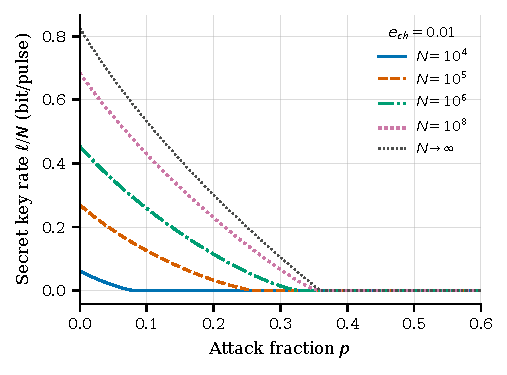
\includegraphics[width=\columnwidth]{figures/fig_rate_vs_p.pdf}
\caption{Secret-key rate versus attack fraction for several block lengths ($\ech=0.01$). The rate reaches zero at $p_{\max}(N)$.}
\label{fig:ratep}
\end{figure}

\begin{table}[!t]
\caption{Largest tolerable IR attack fraction $p_{\max}$ for a positive key}
\label{tab:pmax}
\centering
\small
\begin{tabular}{@{}cccccc@{}}
\toprule
$\ech$ & $N=10^4$ & $10^5$ & $10^6$ & $10^8$ & $N\to\infty$ \\
\midrule
0.00 & 0.116 & 0.293 & 0.360 & 0.389 & 0.392 \\
0.01 & 0.077 & 0.258 & 0.326 & 0.356 & 0.360 \\
0.02 & 0.037 & 0.222 & 0.292 & 0.322 & 0.325 \\
\bottomrule
\end{tabular}
\end{table}


\subsection{Effect of Channel Noise and Minimum Block Length}
Without an attacker, Fig.~\ref{fig:rateE} shows the key rate versus $\ech$. At $N=10^5$ the rate falls from $0.27$ bit/pulse at $\ech=0.01$ to zero near $\ech\approx 0.073$, whereas the asymptotic protocol tolerates $\ech\approx0.098$. Fig.~\ref{fig:nmin} gives the minimum block length. $\Nmin$ is about $2.6\times10^{3}$ at $Q=0$, $2.4\times10^4$ at $5\%$, $1.2\times10^5$ at $7.5\%$, $1.0\times10^6$ at $9\%$, and diverges at the asymptotic limit $Q^\ast$. For links with QBER above about $9\%$, block lengths above $10^6$ are required.

\begin{figure}[!t]
\centering
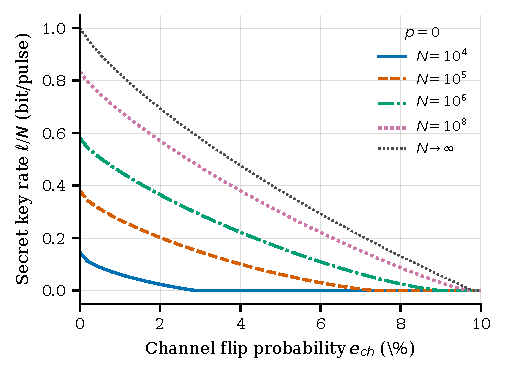
\includegraphics[width=\columnwidth]{figures/fig_rate_vs_e.pdf}
\caption{Secret-key rate versus channel flip probability without eavesdropper ($p=0$).}
\label{fig:rateE}
\end{figure}

\begin{figure}[!t]
\centering
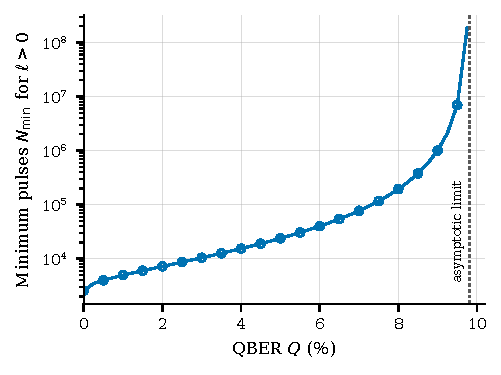
\includegraphics[width=\columnwidth]{figures/fig_nmin.pdf}
\caption{Minimum number of pulses for a positive key as a function of QBER (realised by IR attack with $\ech=0$, i.e.\ $Q=p/4$).}
\label{fig:nmin}
\end{figure}

\subsection{Empirical Validity of the Fluctuation Bound}
To check that \eqref{eq:serfling} is not violated, we sampled the total number of errors on a block of $n+k$ bits with $Q=0.03$, split it at random into a key part ($n$) and a test part ($k$), and estimated $\Pr[Q_n-Q_k\ge\gamma]$ from $4\times10^5$ trials. Table~\ref{tab:tail} shows that the empirical tails lie far below the bound, by at least one order of magnitude, so the bound is valid but conservative at these sizes. This is expected: the bound must hold for every possible $Q$ and for the worst-case distribution, whereas the test uses a single, favourable $Q$. The empirical test cannot probe the tiny probabilities ($\sim10^{-10}$) that the security parameter represents; it can only exclude gross violations.

\begin{table}[!t]
\caption{Empirical tail probability $\Pr[Q_n-Q_k\ge\gamma]$ versus bound \eqref{eq:serfling} ($Q=0.03$)}
\label{tab:tail}
\centering
\small
\begin{tabular}{@{}ccccc@{}}
\toprule
$n$ & $k$ & $\gamma$ & empirical & bound \\
\midrule
500 & 500 & 0.02 & 3.5e-02 & 9.1e-01 \\
500 & 500 & 0.04 & 1.5e-04 & 6.7e-01 \\
500 & 500 & 0.08 & 0.0e+00 & 2.0e-01 \\
2000 & 500 & 0.02 & 6.7e-03 & 8.5e-01 \\
2000 & 500 & 0.04 & 0.0e+00 & 5.3e-01 \\
2000 & 500 & 0.08 & 0.0e+00 & 7.8e-02 \\
5000 & 1000 & 0.02 & 1.4e-04 & 7.2e-01 \\
5000 & 1000 & 0.04 & 0.0e+00 & 2.6e-01 \\
5000 & 1000 & 0.08 & 0.0e+00 & 4.9e-03 \\
\bottomrule
\end{tabular}
\end{table}


\section{Discussion and Limitations}\label{sec:discussion}

\subsection{What the Results Do and Do Not Show}
The finite-key bound \eqref{eq:keylen} holds against arbitrary (coherent) attacks. IR attacks enter the analysis only through the QBER they create. The results therefore answer a design question, namely how much interception a given block length tolerates before the key vanishes, and not a question about the optimality of IR from Eve's point of view.

\subsection{Implications for System Design}
(i) Block lengths below $10^5$ pulses leave little margin: at $N=10^4$ the tolerated attack fraction is below $8\%$ for $\ech=0.01$. (ii) The basis bias $q_X$ should be re-optimised with $N$ and the expected QBER, because it ranges from $0.5$ near threshold to $0.9$ and above for large blocks. (iii) The error-correction efficiency $\fEC$ matters as much as the fluctuation term: in \eqref{eq:asym}, reducing $\fEC$ from $1.16$ to $1.05$ raises the asymptotic QBER tolerance from $9.81\%$ to $10.6\%$.

\subsection{Limitations}
\begin{itemize}
\item \emph{Ideal source and detector.} Multi-photon pulses, loss and dark counts, together with photon-number-splitting attacks \cite{Brassard00,GLLP04}, are not modelled. Real implementations need decoy-state finite-key bounds \cite{Lim14}.
\item \emph{Fixed tolerance rule.} The threshold \eqref{eq:qtol} assumes that the expected QBER is known to the operator; adaptive estimation of $Q$ changes the abort statistics.
\item \emph{Basis-independent noise.} We assumed the same $\ech$ in both bases. Basis-dependent noise requires separate treatment, as the key rate depends on the phase-error rate.
\item \emph{Error-correction model.} $\leakEC=\fEC nh(\Qtol)$ is an idealised model; the leakage of a practical code depends on the code, block length and frame-error rate.
\item \emph{Composability and side channels.} Classical post-processing and authentication costs, and implementation side channels, are not included.
\end{itemize}

\section{Conclusion}\label{sec:conclusion}
We studied the finite-key behaviour of BB84 for error statistics generated by a partial intercept-resend attack in a noisy channel. The QBER obeys $Q=\ech+(1-2\ech)p/4$, which a bit-level simulation reproduces. Combined with a composable key-length bound, this yields explicit values for the key rate, the minimum block length, and the maximal tolerable attack fraction. With $\epssec=10^{-10}$ and $\ech=0.01$, a positive key at $p=0.1$ requires $N\gtrsim1.2\times10^{4}$, and the asymptotic tolerance is approached only for $N\gtrsim10^{8}$. The general-attack bound is conservative against an IR-only adversary by a large margin ($p^\ast\approx0.36$ versus $0.58$), a reminder that security statements must be made against the strongest adversary, while performance targets may be set against realistic ones. Future work will extend the analysis to decoy-state implementations with loss and dark counts, to basis-dependent noise, and to collective attacks tailored to partial information.


\bibliographystyle{IEEEtran}
\bibliography{references}

\end{document}
